\section{Data Driven Drawing}

Our goal is provide a drawing interface on mobile devices that provides the feeling that the user is in full control, while simultaneously providing assistance, in particular, to overcome the inherent fat finger problem. As described earlier, the problem is more constrained than a general drawing system by using a tracing paradigm. The simplest idea would to be to attract drawn strokes to edges found in the image being traced. Unfortunately, this idea fails in two respects. First edge detectors such as Canny methods (see Figure~\ref{fig:edges}, left) have no notion of semantics and thus appear noisy and inconsistent. Second, humans tend to select only the most meaningful edges to draw.

\begin{figure}
  \centering%
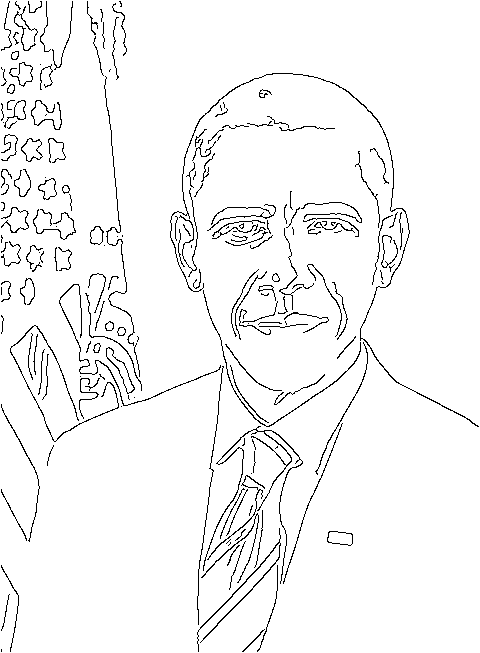
\includegraphics[height=2in]{figures/imagetable/edges_bo.png}
\hspace{0.1in}
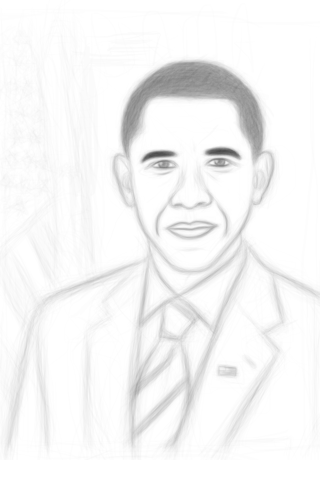
\includegraphics[height=2in]{figures/imagetable/avg_bo.png}
  \caption{Left: Canny edges, Right: average drawing. Neither of these serves as a simple means to correct strokes due to noisy edges (Canny), and fuzzy and inconsistent edges (average).}
  \label{fig:edges}
\end{figure}

To provide assistance, we take advantage of previous drawings of the same face and then pull the users strokes towards a {\em consensus} of previous drawings when the user's stroke appear to approximate the local consensus. The simplest idea for forming a consensus would be to use an {\em average} drawing (see Figure~\ref{fig:edges}, right). This idea is also very problematic as the averages tend to create very fat lines of varying darkness and broad region such as in the hair. Although some kind of {\em skeletonization} may aid the first problem it would fail on the second.

Instead, we develop a stroke correction strategy with two phases.

\textbf{(i) Consensus Finding:} Using the training drawings available for an image, we create a correction vector field, which indicates for each pixel on the image, the delta toward the nearest {\em consensus line}.  This phase is run off-line.

\textbf{(ii) Interactive Correction:} The correction vector field is transmitted to the mobile device along with the image to be traced.  When a user draws a stroke, the field is sampled, and the stroke is moved in a way that maintains the original style.

\subsection{The Correction Vector Field}

%\begin{figure}
%  \centering%
%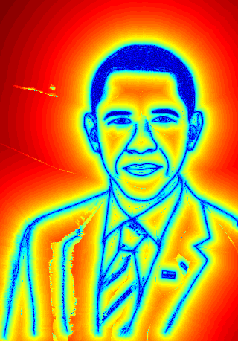
\includegraphics[height=2in]{figures/imagetable/mag_bo.png}
%\hspace{0.1in}
%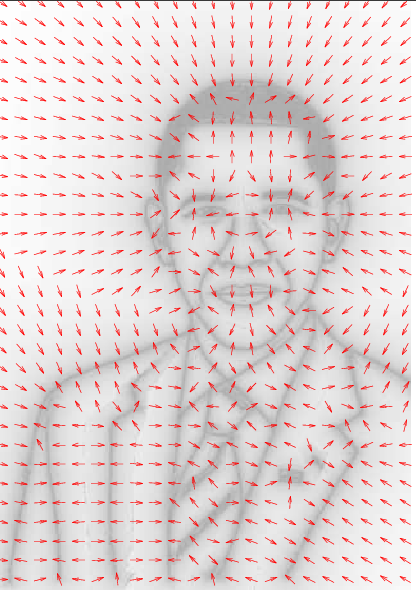
\includegraphics[height=2in]{figures/imagetable/dir_bo.png}
%  \caption{Left: vector magnitude, Right: sampled vector field orientations}
%  \label{fig:vectorfield}
%\end{figure}

A correction vector field, $V(p)$, (see Figure~\ref{fig:image-table}(c)and (d)) is constructed to point, for each location in the image, towards the nearest {\em consensus stroke}, which intuitively represents a stroke that appears in many drawings. Interestingly, we do not need to construct an explicit model of these consensus strokes. Instead, we can directly compute $V$ using a modified version of the {\em mean shift} algorithm~\cite{10.1109/ICCV.1999.790416}.


\begin{figure}
  \centering%
  \includegraphics[width=3.2in]{ellipse.png}
  \caption{A didactic blow-up of the graphs in Figure~\ref{fig:neighbors}. The point at the origin represents a point on a stroke being drawn. The red points are the set of nearest stroke neighbors from database drawings. Note that the orientation of the strokes are always orthogonal to a vector from the origin. We determine a correction vector based on a learned anisotropic Gaussian surrounding a mode of consensus strokes in the database.}
  \label{fig:ellipse}
\end{figure}

\begin{figure}
  \centering%
  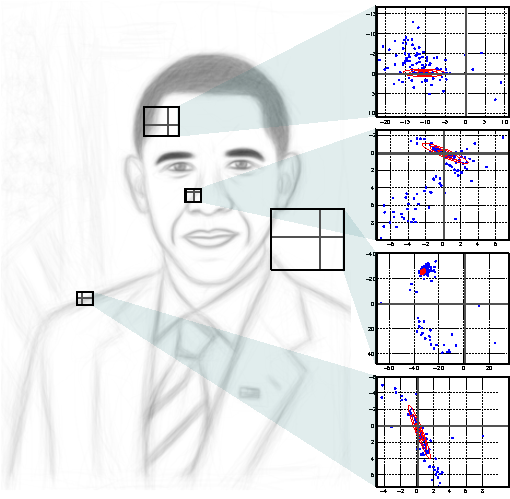
\includegraphics[width=3.2in]{figures/nearest-neighbor-plots.pdf}
  \caption{Nearest neighbors and learned Gaussians for four points in the Obama dataset.  The Gaussian distribution is shown with ellipses at the first, second, and third standard deviations.}
  \label{fig:neighbors}
\end{figure}


Given a point $p$ in the image to be drawn, we first find the nearest stroke point, $v_i$ in each drawing, $D_i$, in our training set. We place the nearest points, $v$, in a coordinate system using $p$ as the origin (see the red points in Figure~\ref{fig:ellipse}). One key observation is that the position of the point $v_i$ also encodes the orientation of the nearest stroke in $D_i$. In particular, the stroke orientation will usually be orthogonal to the vector $v_i$ (aside from minor discretization noise), otherwise there would be some closer stroke point. Thus, a series of nearest strokes that are closely aligned in position and orientation will produce a set of nearest points, $v$, that lie approximately along a line, and this line will intersect the origin (i.e., the point $p$).

Our goal is find a consensus of nearby strokes that avoids undue influence from outliers. For the points, $v$, we seek a {\em mode} in which the points lie in close proximity to each other and lie roughly along a line pointing back towards the origin. We employ an iterative mean shift style algorithm for the mode finding.

Our algorithm works by iteratively updating a vector of weights, {\bf w}, which represent the belief that a particular neighbor is a member of the consensus stroke. The final correction vector, $V(p)$, is given a weighted mean of the points, $v$. We initialize all weights using a symmetric Gaussian centered at the origin, with $\sigma$ equal to the mean distance to all neighbors $v$.


The iteration proceeds by determining an anisotropic Gaussian with weighted mean, $\mu$ (equation~\ref{mean}),
$\sigma_1$ in the direction back toward the origin, $p$, (equation~\ref{sig1}), and ($\sigma_2$) in the orthogonal direction (equation~\ref{sig2}).
\begin{equation}
{\bf \mu} = \left(\sum_j w_j {\bf v}_j\right) / \sum_j w_j  \label{mean}
\end{equation}
and define the normalized mean,
\begin{equation}
{\bf \nu} = \mu/||\mu||
\end{equation}
with the anisotropic standard deviations given by
\begin{eqnarray}
\sigma_1 =  \sqrt{\left(\sum_j w_j (({\bf v}_j-\mu)^{\bf T}\nu)^2\right) / \sum_j w_j} \label{sig1}\\
\sigma_2 =  \sqrt{\left(\sum_j w_j ({\bf v}_j^{\bf T}\nu_\perp)^2\right) / \sum_j w_j} \label{sig2}
\end{eqnarray}
We then reweight all points according to the new gaussian distribution, including a simple regularization $w_i \leftarrow w_i/ (w_i+0.05)$.  The regularization serves to reinforce points near the mean, and further discount points away from the mean. The term 0.05, which intuitively says that any points more than two standard deviations away from the mean are mostly noise, was chosen experimentally.

The system typically converges quickly (all of our experiments use a hard-coded 10 iterations), and $V(p)$ is set to $\mu$.  Examples of nearest neighbor sets and their resulting consensus strokes are shown in Figure \ref{fig:neighbors}.

\subsection{Real-time Stroke Correction}


The vector field, $V$, defined above indicates a best guess of how any individual vertex on a stroke polyline should move to match the consensus of all drawings.

The naive approach is to take the points $(p_1, \ldots, p_k)$ comprising a stroke, along with their correction field samples $(V(p_1), \ldots, V(p_k))$, and directly move each point to arrive at $(p_1 + V(p_1), \ldots, p_k + V(p_k))$.  Unfortunately, noise and discontinuities in the vector field cause undesirable end results. More importantly, any {\em stylistic} choices such as intentional wiggles inherent in the original stroke would also be lost.  To move away from the naive approach, we recognize that the fat finger problem is likely to cause the input stroke to be off by a roughly constant displacement, while the original stroke shape is likely to represent the user's {\em intent}.

Our goal is thus to use the guidance of the vector field on where to move, but still maintain most of the shape of the original stroke.  We therefore create and solve an over-constrained linear system that represents both of those objectives.

With $p_i$ representing input stroke sample locations for $i=1\ldots k$, $V_i$ a shorthand for $V(p_i)$ representing the correction vector field at $p_i$, and $p_i'$ representing the corrected samples, we construct a quadratic error function as:

\begin{equation}
E = \alpha \sum_{i=1}^k (p_i' - (p_i + V_i))^2 +  \sum_{i=2}^k ((p_i' - p_{i-1}') - (p_i - p_{i-1}))^2
\end{equation}

The first term represents the faithfulness to the correction vector field. The second term tries to maintain the shape of the stroke by enforcing that neighboring points move in sync. The $\alpha$ term weights the relative importance of the two terms. The error is minimized with a standard least squares solver on the $2k-1$ terms.

\subsubsection{Setting $\alpha$ - Closely Spaced Consensus Strokes}

A higher $\alpha$ value results in {\em stiffer} strokes in the sense that they maintain their shape instead of following variations in the vector field precisely. Aside from maintaining the {\em style} of the strokes, a high stiffness also help avoid having part of a stroke pulled in one direction and another part pulled in another. This can happen especially when there are two closely space parallel lines in the consensus, such as the two sides of the nose, or the bottom and top of the lips. Unfortunately, a very high $\alpha$ does not allow the strokes to adapt at all to the subtleties of the consensus drawing represented in the vector field.

To achieve the goals of avoiding the two nearby stroke problem while balancing stiffness and style, we use a {\em continuation method}, performing three iterations of the solver described above. We begin with $\alpha=10$. This high stiffness value leads to an almost rigid transformation of the stroke. We then lower $\alpha$ to 7, and feed the previous result, $\hat{p}$ into the first error term, $(p_i' - (\hat{p}_i + V_i))$, while keeping the original terms for the latter half of the error measure, and solve the new system. We repeat this one final time with $\alpha=4$ to get our final result. The $\alpha$ values (10,7,4) were chosen experimentally.

\subsubsection{Purely Stylistic Strokes}

We also found that some strokes are purely stylistic in nature. For example, some writes ``Obama'' above the president's head. We do not want such strokes to have parts pulled towards the consensus. We make a binary decision about whether the stroke is purely stylistic, in which case, we leave it alone. A stroke is defined to be purely stylistic if either of two conditions is met. Either the maximum vector length, $\max_i||V(p_i)||$, is greater than $5mm$ (approximately $1/10^{th}$ the screen width), or a stroke's direction is mostly orthogonal to the vector field. The latter term is measured with the average of absolute cosines $\frac{1}{N}\sum_i||N(p_i - p_{i-1}) \cdot N(V(p_i))||\textrm{,}$ where $N(\cdot)$ normalizes vectors. If the average falls below 0.5, the stroke is considered purely stylistic.





